    \documentclass[12pt,a4paper]{article}
    \usepackage[T2A]{fontenc}
    \usepackage[utf8]{inputenc}
    \usepackage[russian]{babel}
    \usepackage{amsmath}
    \usepackage{amssymb}
    \usepackage{graphicx}
    \usepackage{floatrow}
    \usepackage{booktabs}
    \usepackage{wrapfig}
    \usepackage{lipsum}
    \usepackage{subcaption}
    \usepackage{fancyhdr}
    \usepackage{mathrsfs}
    \usepackage{tikz}

    \usepackage{graphicx, scalerel}
    \usepackage[warn]{mathtext}
    \usepackage{indentfirst}
    \usepackage[margin = 25mm]{geometry}
    \usepackage{caption}
    \usepackage{multirow}
    \usepackage{gensymb}
    
    \newcommand{\figref}[1]{(См. рис. \ref{#1})}
    \newcommand{\secref}[1]{(См. раздел. \ref{#1})}
    
    \newcommand{\e}[1]{\text{$\cdot10^{#1}$}}
    
    \pagestyle{fancy}
    \fancyhead{}
    \fancyhead[L]{Работа 4.5.2}
    \fancyhead[R]{}
    \fancyfoot[C]{\thepage}
    
    \author{\normalsize Выполнил: Голубович Тимур, группа Б01-108 \\
    	\normalsize 27.04.2023}
    \date{}
    
    \usepackage{float}
    \restylefloat{table}
    \title{
    	\large Отчет о выполнении лабораторной работы 4.5.2 \\
    	\Large Интерференция лазерного излучения
     }
    
    \begin{document}
    	\maketitle
    	
    \section*{Цель работы}
    Исследование видности интерференционной картины излучения гелий-неонового лазера и определение длины когерентности излучения.
    
    \section*{Оборудование и приборы} 
    He-Ne-лазер; интерферометр Майкельсона с подвижным зеркалом; фотодиод с усилителем; осциллограф; поляроид; линейка.

	
\section*{Теоретическое введение}

	Важный параметр интерференционной картины --- ее видность:

    \begin{equation}\label{V0}
    V = \dfrac{I_{max} - I_{min}}{I_{max} + I_{min}}
    \end{equation}
    
    Удобно представлять видимость в виде произведения функций различных параметров установки/системы:
    
    \begin{equation}\label{VVV}
    V = V_1 V_2 V_3
    \end{equation}
    
    Рассмотрим эти функции подробнее. Первая из них отвечает за отношение интенсивностей интерферирующих волн:
    
    \begin{equation}\label{V1}
    V_1 = \dfrac{2\sqrt{\delta}}{1 + \delta}, \quad \delta = \dfrac{B_m^2}{A_m^2}
    \end{equation}
    
    
    Здесь $ A_m, B_m $ --- амплитуды волн. Вторая функция учитывает влияние разности хода и спектрального состава волн:
    
    
    \begin{equation}\label{}
    \gamma_2 = \dfrac{\sum\limits_n A_n^2 \cos{\dfrac{2\pi \Delta \nu n l}{c}}}{\sum\limits_n A_n^2} \sim e^{-(\pi \Delta F l /c^2)}
    \end{equation}
    
    \begin{wrapfigure}{l}{0.35\linewidth} 
    	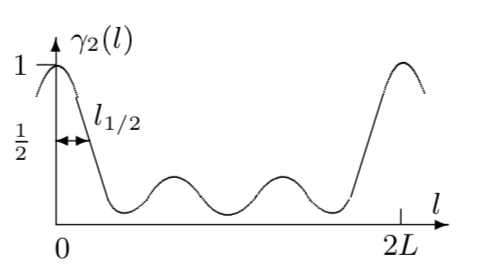
\includegraphics[width=\linewidth]{res/v2.png}
    	\caption{Качественный график $ V_2 $}
    	\label{V2graf}
    \end{wrapfigure}
    
    
    Здесь $ l $ --- разность хода, $ \Delta\nu $ --- спектральный состав излучения, $ A_n^2 $ --- интенсивность мод. Оценка приведена из перехода к непрерывному пределу. На графике (рис.\ref{V2graf}) показан вид $ V_2(l) $, позволяющий получить расстояние $ L $ между зеркалами резонатора и межмодовое расстояние $ \Delta \nu $. Величина $ l_{1/2} $  позволяет оценить диапазон частот $ \Delta F $.
    Формулы связи межмодового расстояния и длины $ L $, а также $ l_{1/2} \; \text{и} \; \Delta F $ таковы:
    
    \begin{equation}\label{dnu}
    \Delta \nu = \dfrac{c}{2L}, \quad l_{1/2} \approx \dfrac{0.26 c}{\Delta F}
    \end{equation}
    
    Последняя функция --- зависимость от угла поляризации $ \alpha $:
    
    \begin{equation}\label{}
    V_3 = |\cos{\alpha}|
    \end{equation}

	
	\section*{Экспериментальная установка}

    Для получения интерференционной картины используется интерферометр Майкельсона, смонтированный на вертикально стоящей массивной металлической плите. Схема установки приведена на рисунке.
    
    \begin{figure}[h!]
    	\centering
    	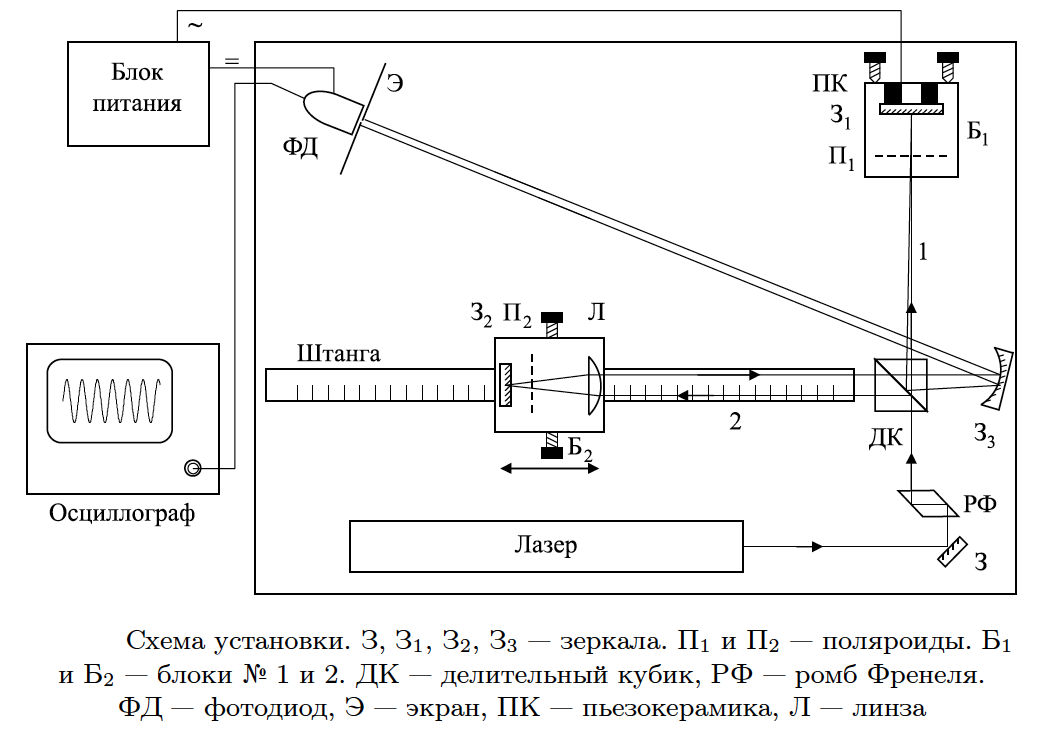
\includegraphics[width=\linewidth]{res/lab.png}
    	\caption{Экспериментальная установка}
    	\label{lab}
    \end{figure}

    Источником света служит гелий-неоновый лазер (средняя длина
    волны $ \lambda_0 = 632.8 $ нм). Пучок лазерного излучения отражается от зеркала З и проходит призму полного внутреннего отражения РФ (ромб Френеля), которая превращает линейную поляризацию излучения в круговую. Если в установке используется лазер, излучающий неполяризованный свет, то ромб Френеля не нужен, но он и не мешает выполнению
    работы. Далее лазерное излучение делится диагональной плоскостью
    делительного кубика ДК на два пучка.
    
    \begin{wrapfigure}{l}{0.35\linewidth} 
    	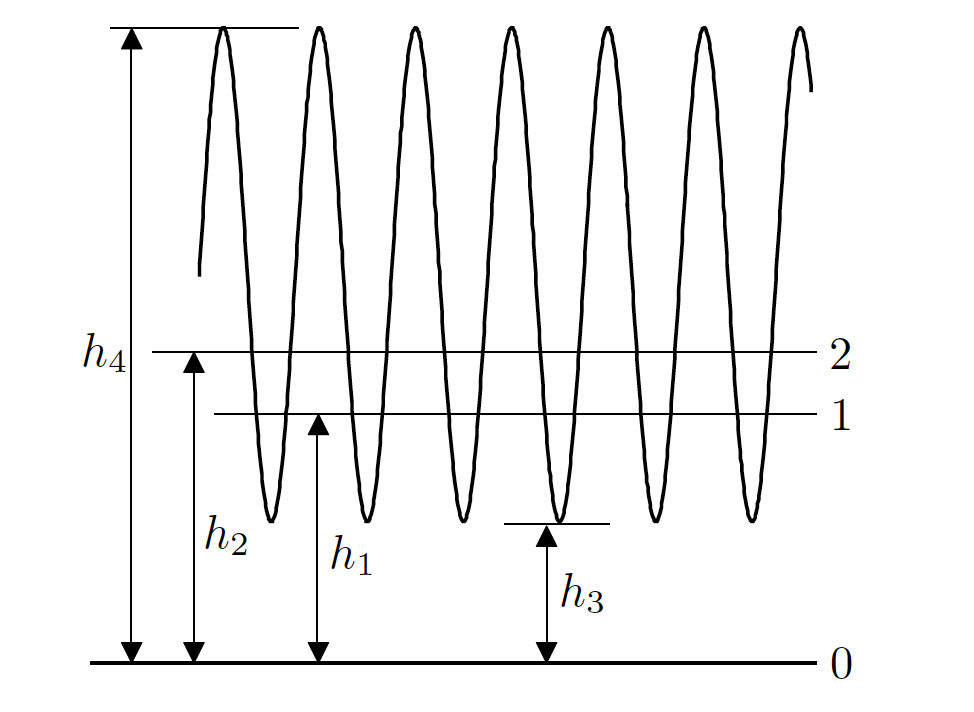
\includegraphics[width=\linewidth]{res/os}
    	\caption{Сигнал фотодиода на осциллографе}
    	\label{}
    \end{wrapfigure}
    
    Осциллограф мы используем для нахождения следующих величин: фоновой засветки (линия 0 --- перекрыты оба пучка 1 и 2); интенсивность света каждого из пучков (линии 1 или 2 --- перекрыт пучок
    2 или 1); максимума и минимума интенсивности интерференционной
    картины (открыты оба пучка). При этом параметр $ \delta $ из \eqref{V1},  определяется отношением
    
    \begin{equation}\label{delta}
    \delta = \dfrac{h_1}{h_2}
    \end{equation}
    
    Понятно, что из физического смысла, наша видимость рассчитывается очевидным образом, согласно формуле \eqref{V0}, так:
    
    \begin{equation}\label{V}
    V = \dfrac{h_4 - h_3}{h_4 + h_3}
    \end{equation}
    
    Отсюда, используя \eqref{VVV}, мы можем получить наши функции из \eqref{V}, фиксируя одну из них (т.е. беря равной единице). Так, при $ \alpha = 0 \Rightarrow V_3 = 1 $, 
    
    \begin{equation}\label{V2}
    V_2 (l) = \dfrac{V}{V_1} = \dfrac{h_4 - h_3}{h_4 + h_3} \cdot \dfrac{h_2}{h_1}
    \end{equation}
    
    А приняв разность хода $ l = 0 \Rightarrow V_2 = 0 $, можно найти 
    
    \begin{equation}\label{V_3}
    V_3(\alpha) = \dfrac{V}{V_1} = \dfrac{h_4 - h_3}{h_4 + h_3} \cdot \dfrac{h_2}{h_1}
    \end{equation}
	
    \section*{Ход работы}
	

    \subsection*{Изучение поляризации}
    
    Поворотами поляризатора $ \text{П}_1 $ убедимся, что свет от лазера --- поляризованный. Настроив поляроид на минимальную видимость и введя дополнительный поляроид, мы вновь получаем интерференционную картину при его поворотах. Интенсивность излучения при вращении поляроида меняется, что говорит о его \textbf{не хаотической} поляризации. При вращении также изменяется интерференционная картина, что говорит о \textbf{линейной или круговой} поляризации, а не хаотической.


    \subsection*{Измерение зависимости видности от угла}
    
    Исследуем зависимость видности интерференционной картины от угла
    $ \alpha $ поворота поляроида $ \text{П}_1 $ при нулевой разности хода ($ V_2 = 1 $). Для этого измерим величины $ h_1, h_2, h_3 \; \text{и} \; h_4 $ на экране осциллографа. Результаты занесем в таблицу \ref{table_v3} и построим график согласно формуле \eqref{V_3}. Значения для $ \delta, V, V_1 $ получим из формул выше.

     \begin{table}[h!]
       \centering
       \footnotesize
       \begin{tabular}{cccccc}
\toprule
$\beta, {^\circ}$ & $h_1$, дел & $h_2$, & $h_3$, дел & $h_3$, дел & $V_3$ \\
\midrule
90 & 1.0 & 4.1 & 4.6 &  6.1 & 0.177 \\
80 & 1.2 & 4.1 & 3.5 &  7.2 & 0.413 \\
70 & 1.5 & 4.1 & 2.6 &  9.0 & 0.623 \\
60 & 2.0 & 4.1 & 1.8 & 10.5 & 0.753 \\
50 & 2.8 & 4.0 & 1.0 & 13.0 & 0.871 \\
40 & 4.2 & 4.2 & 0.9 & 16.1 & 0.894 \\
30 & 5.0 & 4.1 & 0.8 & 17.0 & 0.915 \\
20 & 6.4 & 4.1 & 1.2 & 20.0 & 0.909 \\
10 & 5.6 & 4.2 & 1.4 & 23.1 & 0.895 \\
0  & 6.6 & 4.3 & 2.0 & 24.6 & 0.869 \\
\bottomrule
\end{tabular}
       \caption{Измерение зависимости $V_3$ от $\beta$}
       \label{table_v2}
    \end{table}	


    \begin{figure}[h!]
        \centering
        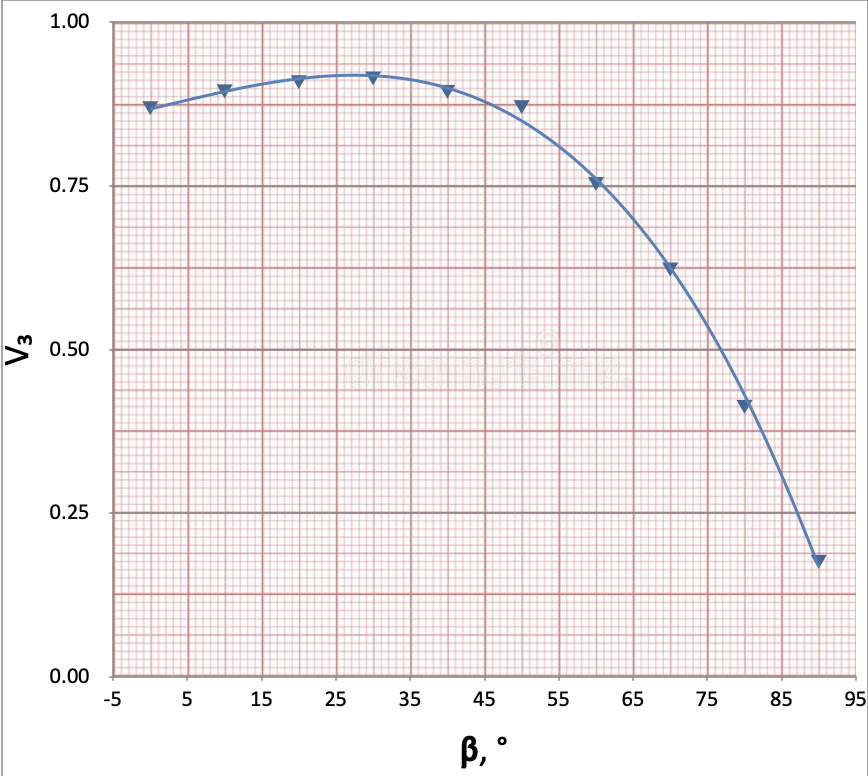
\includegraphics[width=0.8\linewidth]{src/v3b.png}
        \caption{График зависимости $V_3 (\beta)$}
    \end{figure}

    Из графика следует, что он приближается функцией $ \cos^2 \alpha $. Это значит, что \textbf{поляризация --- линейная}. Выполняется \textbf{закон Малюса}:
    \[ I = I_0 \cos^2\alpha \]

    \subsection*{Измерение зависимости видности от дальности хода}

    Теперь установим $ \alpha $ на максимальную видность и будем перемещать блок $ \text{Б}_2 $, тем самым изменяя дальность хода $ x $. Аналогично предыдущему пункту измерим величины $ h_1, h_2, h_3 \; \text{и} \; h_4 $ на экране осциллографа. Результаты занесем в таблицу \ref{table_v2} и построим график согласно формуле \eqref{V2}. Значения для $ \delta, V, V_1 $ получим из формул выше.

     \begin{table}[h!]
       \centering
       \footnotesize
       \begin{tabular}{cccccc}
\toprule
$x, см$ & $h_1$, дел & $h_2$, & $h_3$, дел & $h_3$, дел & $V_2$ \\
\midrule
10 & 4.5 & 5.5  & 3.7  & 16.1 & 0.629 \\
12 & 4.5 & 7.0  & 3.2  & 19.5 & 0.736 \\
14 & 4.5 & 8.9  & 3.1  & 23.1 & 0.808 \\
16 & 4.5 & 7.1  & 2.3  & 20.6 & 0.820 \\
18 & 4.6 & 9.5  & 3.7  & 24.0 & 0.782 \\
20 & 4.7 & 6.8  & 3.1  & 18.8 & 0.729 \\
24 & 4.7 & 11.0 & 8.5  & 22.0 & 0.483 \\
28 & 4.6 & 12.0 & 13.0 & 18.8 & 0.204 \\
34 & 4.1 & 7.8  & 10.6 & 12.8 & 0.099 \\
40 & 4.1 & 11.0 & 13.2 & 15.9 & 0.104 \\
50 & 2.0 & 4.5  & 6.0  & 7.1  & 0.091 \\
60 & 5.0 & 12.3 & 16.4 & 18.2 & 0.057 \\
70 & 3.0 & 11.0 & 9.4  & 17.2 & 0.357 \\
74 & 3.0 & 10.6 & 7.5  & 19.0 & 0.523 \\
76 & 4.0 & 13.2 & 7.0  & 28.0 & 0.710 \\
78 & 4.1 & 10.5 & 4.5  & 25.0 & 0.773 \\
80 & 4.8 & 13.5 & 4.8  & 31.0 & 0.832 \\
82 & 4.9 & 8.5  & 3.0  & 23.0 & 0.799 \\
84 & 5.0 & 16.7 & 7.9  & 34.6 & 0.746 \\
86 & 3.1 & 12.5 & 7.5  & 23.3 & 0.643 \\
88 & 3.1 & 10.0 & 7.4  & 18.6 & 0.507 \\
\bottomrule
\end{tabular}

       \caption{Измерение зависимости $V_2$ от $x$}
       \label{tab:t1}
    \end{table}	


    \begin{figure}[h!]
        \centering
        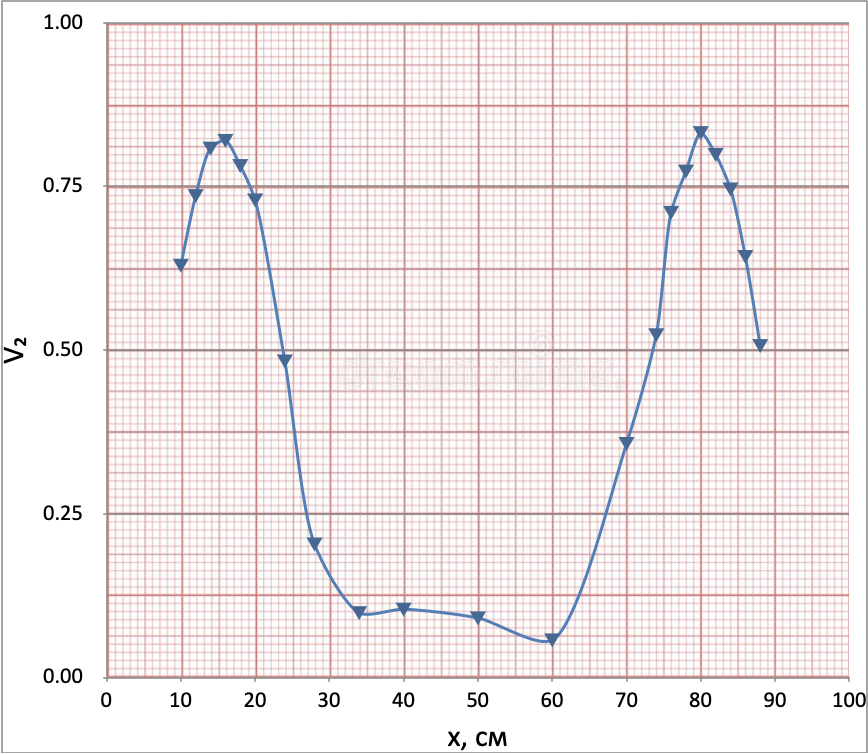
\includegraphics[width=0.8\linewidth]{src/v2x.png}
        \caption{График зависимости $V_2 (x)$}
    \end{figure}


    Видно, что у нас наблюдается 2 максимума по краям области измерения и некоторые колебания в промежуточной области. А именно, максимумы в области $ x_1 \approx (16 \pm 1) \; \text{см} $ и в области $ x_2 \approx (80 \pm 1) \; \text{см} $, откуда получаем следующий результат:
    
    \begin{equation}\label{}
    L = \dfrac{1}{2} (x_2 - x_1) = (32.0 \pm 1.2) \; \text{см}
    \end{equation}
    
    Отсюда нетрудно получить и значение $ \Delta \nu $ из формулы \eqref{dnu}:
    
    \begin{equation}\label{}
    \Delta \nu = \dfrac{c}{2L} \approx (4.7 \pm 0.2) \cdot 10^8 \; \text{Гц}
    \end{equation}
    
    Оценим $ l_{1/2} \approx \cdot(80 - 72) \text{ см} = (8 \pm 2) \text{ см} $, откуда по формуле \eqref{dnu} получаем
    
    \begin{equation}\label{}
    2\Delta F = 2\cdot \dfrac{0.26 c}{l_{1/2}} \approx (19.5 \pm 4.9) \cdot 10^8 \; \text{Гц}
    \end{equation}
    
    Тогда для числа одновременно генерируемых лазером продольных волн можно провести оценку:
    
    \begin{equation}\label{}
    N \approx 1 + \dfrac{ 2\Delta F}{\Delta \nu} \approx 5 \pm 1
    \end{equation}

	\vfill
	\section*{Вывод}
    \begin{itemize}
        \item В ходе выполнения лабораторная работы была изучена поляризация излучения лазера. При этом было установлено, что при вращении поляроида интенсивность излучения меняется, что говорит о его не хаотической поляризации. При этом изменяется и интерференционная картина. По этим результатам можно предположить, что поляризация \textbf{линейная} или \textbf{круговая}.
        \item Затем была исследована зависимость видности интерференционной картины от угла поляроида $ \text{П}_1 $. Из результатов измерений и аппроксимации следует, что зависимость приближается функцией $ \cos^2 \alpha $. Это значит, что поляризация излучения --- \textbf{линейная} согласно закону Малюса.
        \item В заключительной части работы была исследована зависимости видности интерференционной картины от разности хода. По полученным данным было оценено расстояние между максимумами, расстояние $ L $ между зеркалами оптического резонатора лазера, а также межмодовое расстояние $ \Delta\nu $. Для этих величин были получены следующие результаты:
        \[ \boxed{L = (32.0 \pm 1.2) \text{ см}} \]
        \[ \boxed{\Delta\nu = (4.7 \pm 0.2) \cdot 10^8 \text{ Гц}} \]
        \item Также по графику также было оценена полуширина $ l_{1/2} $. При помощи этих данных было получен диапазон частот $ 2\Delta F $, в котором происходит генерация продольных мод, и приблизительное число мод. Были получены следующие результаты:
        \[ \boxed{l_{1/2} = (8 \pm 2) \text{ см}} \]
        \[ \boxed{2\Delta F = (19.5 \pm 4.9)\cdot 10^8 \text{ Гц}} \]
        \[ \boxed{N = 5 \pm 1} \]
        \item Основной вклад в погрешнсть в ходе выполнения работы могла внести ошибка при определении продольного сдвига второго зеркального блока. Также не всегда было реальным точное измерение максимумов напряжений по показаниям осциллографа в силу их изменения во времени.
    \end{itemize}

\newpage
\begin{thebibliography}{9}
	\bibitem{Siv} Сивухин Д. В. \emph{Общий курс физики. Том 4 Оптика}, 2004
	\bibitem{kirich} Кириченко Н.А. \emph{Оптика.}, 2011
	\bibitem{max} \emph{Лабораторный практикум по общей физике. В 3 томах. Том 3. Оптика: учебное пособие} под ред. А. В. Максимычева, М. Г. Никулина
\end{thebibliography}

\end{document}
